\documentclass[letterpaper,10pt,twocolumn,titlepage]{article}

\usepackage{graphicx}                                        
\usepackage{amssymb}                                         
\usepackage{amsmath}                                         
\usepackage{amsthm}                                          

\usepackage{alltt}                                           
\usepackage{float}
\usepackage{color}
\usepackage{url}

\usepackage{balance}
\usepackage[TABBOTCAP, tight]{subfigure}
\usepackage{enumitem}
\usepackage{pstricks, pst-node}


\usepackage{geometry}
\geometry{textheight=8.5in, textwidth=6in}

%random comment

\newcommand{\cred}[1]{{\color{red}#1}}
\newcommand{\cblue}[1]{{\color{blue}#1}}

\usepackage{hyperref}
\usepackage{geometry}

\def\name{Jonah Brooks}

%% The following metadata will show up in the PDF properties
\hypersetup{
  colorlinks = true,
  urlcolor = black,
  pdfauthor = {\name},
  pdfkeywords = {cs311 ``operating systems'' files filesystem I/O},
  pdftitle = {CS 311 Project 1: UNIX File I/O},
  pdfsubject = {CS 311 Project 1},
  pdfpagemode = UseNone
}

\begin{document}

\begin{figure}[h]
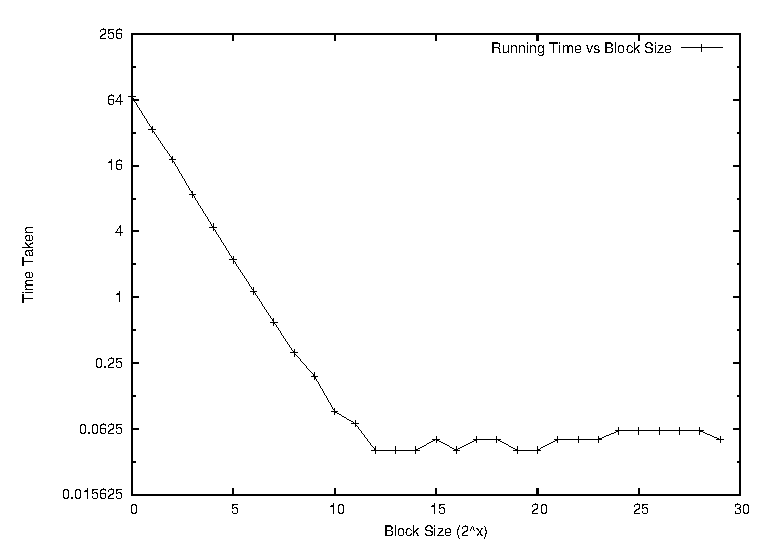
\includegraphics{graph.eps}  
\end{figure}

This is the write-up for assignment 1 of CS311. 
In this assignment, I created a program (h1.cpp) to copy an abitrary file using various block sizes. 
Printing out the time it took to copy for each block size allowed me to create a graph (included above).

\section{Design Decisions}
I chose to time my code using the clock function of ctime since I wanted to increment the block size within my code.
This allowed me to keep most of my work within one file, rather than manually collecting data for each block size.
I tried various timing techniques, including functions from sys/time, sys/times, and other functions from ctime.
The clock function seemed to be the most elegant of the lot, so I chose it for timing my code.

As for the block size increments, I chose powers of two, since they would be more likely to match the system's natural block size.
When outputting the data, I took the base two log of the block size, since the numbers get rather large.

\vfill\break

\hfill Jonah Brooks

\hfill CS311 HW1

\hfill 01-23-2012

\vspace*{2.9in}

\section{Commit Log}
\input{git_log}

\end{document}
